\documentclass[a4paper, 10pt]{article}

\usepackage{hyperref}
\usepackage[utf8]{inputenc}
\usepackage[french]{babel}
\usepackage{eurosym} % \oe{} ...
\usepackage{graphicx}
\usepackage[T1]{fontenc}
\usepackage{geometry}
\usepackage{fancyhdr}
\usepackage{lastpage}
\usepackage{paralist}
\usepackage{listings}
\usepackage{color}
\usepackage{amsmath}

\lstset{language=Java, frame=shadowbox, rulesepcolor=\color{black}}

\geometry{hmargin=1.5cm, vmargin=2cm }
\pagestyle{fancy}
\setlength\parindent{0pt}

\lhead{\'Ecole des Mines de Douai -- Mineur MAD} \lfoot{G.L.}
\rhead{TD/TP 01 - Décisions sous incertitude}
\rfoot{Page : \thepage/\pageref{LastPage}}
\cfoot{} \chead{}

\newcounter{QQ}

\newcommand{\question}[1]{ \medskip \sffamily \textsc{\textbf{\large Question \stepcounter{QQ} \arabic{QQ}} \emph{\small(#1)}} : }

\begin{document}
\author{\'Ecole des Mines de Douai -- FI 2A}
\date{}
\title{\Large{\textbf{Exam - Décisions sous incertitude \\ Troll}}}
\maketitle
\thispagestyle{fancy}

% \section*{Nom(s) et prénom(s): \_\_\_\_\_\_\_\_\_\_\_\_\_\_ $\quad$ \_\_\_\_\_\_\_\_\_\_\_\_\_\_}

\bigskip

% Le barème est indicatif et sera ajusté lors de la correction.

\section*{Retro-engineering}

You are in possession of the next script describing the behavior of a Troll in a video game. You aim to understand this behavior.

\begin{lstlisting}[caption={Script}]
  String behavior( int [] s )
  if( s[0] == 1 )
  {
    if( s[1] == 1 )
      return "run away";
    else
      return "attack";
  }
  else
  {
    if( s[1] < 3 )
      return "sleep";
    else
    {
      if( s[2] == 0 )
        return "explore";
      else
        return "socialize";
    }
  }
\end{lstlisting}

\question{3 points} Build the decision-tree matching the Troll behavior.

\question{1.5 points} Enumerate the variables and their possible domains according to the Troll behavior.

\question{0.5 point} What is the state-space size covered by the decision-tree ?

\question{1 point} What is the action returned by the state $[1,\ 2,\ 1]$ ?

\question{1 point} How many states share the same leaf node as the state $[1,\ 2,\ 1]$ ? (equation and result)
  
\question{1 points} Propose coherent name to each of the state variables with a short justification. 


\section{Probabilities on attack outcome }
  
  We aim to model a combat between a Troll and a Knight in order to increase the behavior of the Troll.
  The Troll and the Knight have both a health level starting from $3$ down to $0$ ($3$: healthy ; $2$: hurt ; $1$: dying ; $0$: dead).
  During Troll attack, the Troll can potentially hit the Knight and reduce its health level by $1$ to $3$ damages.
  In normal condition the troll have $0.1$ chance to hit with $1$ damage, $0.4$ chance to hit with $2$ damages and $0.2$ chance to hit with $3$ damages, otherwise the Knight evade from the attack.
  If the health of the Troll is reduced the chances to hit are reduced to half their values for each damage the Troll have taken.
  Furthermore the Knight potentially use a shield, in this case, the damage is reduced by $1$.

\question{2 points}
  Propose a Bayesian network allowing to compute the damage a Troll could do during an attack.
  
\question{2 points}
  Give table of the condition probabilities attached to the node modeling the damage a Troll made.

\question{1 points}
  Considering that the Troll is healthy and half of Knights use shields, what is the probability that the Troll kill the Knight at the first attack ?

\question{2 points}
  A combat between a Troll and a Knight is composed of several Troll attacks, where the Knight can counter attack if he is alive and if he gets no damages (he successfully evade the Troll or the shield absorbs all damages).
  Counter attack make $1$ damage with a probability of $0.5$ and $2$ with a probability of $0.2$ what ever the health levels of the Knight and the Troll.
  Finally, the Knight damage is increased by $1$ if he doesn't use a shield (which mean he is better armed).
  Propose a new Bayesian networks modeling the evolution of the Troll and Knight health.

\question{1 points} What is the name of this kind of Bayesian networks ?

\question{3 points}
  Implement, in Java language style, the function returning the probabilities on the Troll health evolution according to your Bayesian network.
  The function take as parameters all the variables needed to compute the probabilities (several integers with appropriate names) and return a table of $4$ probabilities (one for each of the $4$ possible health levels).
  Example of expected function signature (with \emph{avn} for appropriate variable name)  : 
  $$ \text{\emph{ double [] trollHealthEvolution( int avn1,  int avn2,  int avn3, [...] ) }} $$

\section{Markov Decision Process}
  
  Based on the Bayesian network we propose to develop a Markov decision process modeling a combat between the Troll and a Knight armed with a shield.
  The states are only composed by the health of the Troll and the Knight plus three extra states modeling that the Troll is dead, the Knight is dead and the combat is over.
  The decision for the Troll consists in attacking or running away.
  The action ``run away'' always falls down the state \emph{End} with a probability of $1.0$.
  The transition of action ``attack'' is modeled by the bottom figure. 
  The model have $12$ states and $2$ actions.
  The reward function model the pleasure the Troll has when it attacks and kills the Knight.
  
  $$ r(s, a)= \left\{
  \begin{array}{r l}
      -10  & \text{if Troll is dead} \\
      8    & \text{if Knight is dead} \\
      0    & \text{if combat is ended} \\
      2    & \text{if Troll is attacking (combat not ended and Troll or Knight not dead)} \\
      0    & \text{if Troll is running away}
   \end{array}
   \right.$$

   \begin{figure}[!b]
    \centering
    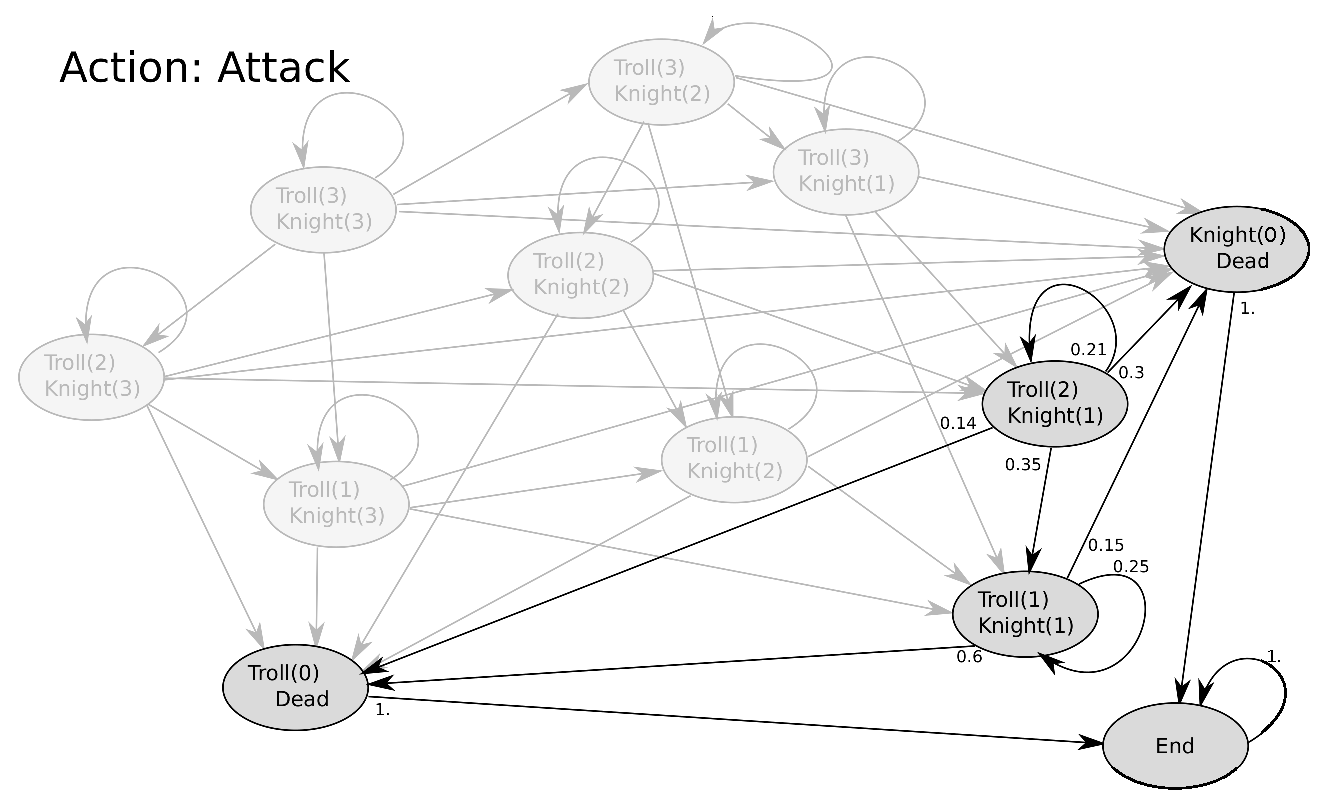
\includegraphics[width=0.68\textwidth]{fig/Attacking}
    \caption{Transition function for the ``attack'' action (highlighted on states pointed by questions 13 and 14)}
   \end{figure}

\question{1 points}
  Considering the Bellman Equation what is the best action and its associated value at time-step $t=1$ for all the $5$ states:
  (\emph{End} ; \emph{Troll(0)} ; \emph{Knight(0)}
  \emph{Troll(2)-Knight(1)} ; \emph{Troll(1)-Knight(1)}.
  $$ \text{Bellman equation:} \qquad V_t(s)= \max_{a}\left(r(s,\ a) + \sum_{s'\in S} t(s,\ a,\ s') V_{t-1}(s') \right) \quad \text{with} \quad V_0(s)= 0  $$
\question{2 points} Same question at time-step $t=2$.



\end{document}